%% BioMed_Central_Tex_Template_v1.06
%%                                      %
%  bmc_article.tex            ver: 1.06 %
%                                       %

%%IMPORTANT: do not delete the first line of this template
%%It must be present to enable the BMC Submission system to
%%recognise this template!!

%%%%%%%%%%%%%%%%%%%%%%%%%%%%%%%%%%%%%%%%%
%%                                     %%
%%  LaTeX template for BioMed Central  %%
%%     journal article submissions     %%
%%                                     %%
%%          <8 June 2012>              %%
%%                                     %%
%%                                     %%
%%%%%%%%%%%%%%%%%%%%%%%%%%%%%%%%%%%%%%%%%


%%%%%%%%%%%%%%%%%%%%%%%%%%%%%%%%%%%%%%%%%%%%%%%%%%%%%%%%%%%%%%%%%%%%%
%%                                                                 %%
%% For instructions on how to fill out this Tex template           %%
%% document please refer to Readme.html and the instructions for   %%
%% authors page on the biomed central website                      %%
%% http://www.biomedcentral.com/info/authors/                      %%
%%                                                                 %%
%% Please do not use \input{...} to include other tex files.       %%
%% Submit your LaTeX manuscript as one .tex document.              %%
%%                                                                 %%
%% All additional figures and files should be attached             %%
%% separately and not embedded in the \TeX\ document itself.       %%
%%                                                                 %%
%% BioMed Central currently use the MikTex distribution of         %%
%% TeX for Windows) of TeX and LaTeX.  This is available from      %%
%% http://www.miktex.org                                           %%
%%                                                                 %%
%%%%%%%%%%%%%%%%%%%%%%%%%%%%%%%%%%%%%%%%%%%%%%%%%%%%%%%%%%%%%%%%%%%%%

%%% additional documentclass options:
%  [doublespacing]
%  [linenumbers]   - put the line numbers on margins

%%% loading packages, author definitions

\documentclass[twocolumn]{bmcart}% uncomment this for twocolumn layout and comment line below
%\documentclass{bmcart}

%%% Load packages
%\usepackage{amsthm,amsmath}
%\RequirePackage{natbib}
%\RequirePackage[authoryear]{natbib}% uncomment this for author-year bibliography
%\RequirePackage{hyperref}
\usepackage[utf8]{inputenc} %unicode support
%\usepackage[applemac]{inputenc} %applemac support if unicode package fails
%\usepackage[latin1]{inputenc} %UNIX support if unicode package fails


\usepackage{booktabs} % For formal tables
\usepackage{graphicx}
\usepackage{xspace}

\usepackage{lstcustom}




%%%%%%%%%%%%%%%%%%%%%%%%%%%%%%%%%%%%%%%%%%%%%%%%%
%%                                             %%
%%  If you wish to display your graphics for   %%
%%  your own use using includegraphic or       %%
%%  includegraphics, then comment out the      %%
%%  following two lines of code.               %%
%%  NB: These line *must* be included when     %%
%%  submitting to BMC.                         %%
%%  All figure files must be submitted as      %%
%%  separate graphics through the BMC          %%
%%  submission process, not included in the    %%
%%  submitted article.                         %%
%%                                             %%
%%%%%%%%%%%%%%%%%%%%%%%%%%%%%%%%%%%%%%%%%%%%%%%%%
%\def\includegraphic{}
%\def\includegraphics{}



%%% Put your definitions there:
\startlocaldefs
\lstdefinelanguage{Xtext}[]{Java}{
	morekeywords={grammar, with, hidden, generate, as, import, returns, current, terminal, enum},
	keywordstyle=[2]{\textbf},
	morestring=[b]",
	tabsize=3
}
\newcommand{\lstXtext}[1]{\lstinline[breaklines=true,language=Xtext,basicstyle=\listingsfontinline,mathescape,literate={\-}{}{0\discretionary{-}{}{}}]\S#1\S}


\lstdefinelanguage{DRL}[]{Java}{
	morekeywords={rule, when, from, accumulate, and, in, then, for, int, end},
	keywordstyle=[2]{\textbf},
	morecomment=[l]{//}, 
	morecomment=[s]{/*}{*/}, 
	morestring=[b]",
	tabsize=2
}

\lstdefinelanguage{Freemarker}[]{Java}{
	morekeywords={if, assign, else},
	keywordstyle=[2]{\textbf},
	morecomment=[l]{//}, 
	morecomment=[s]{/*}{*/}, 
	morestring=[b]",
	showspaces=false,
	tabsize=2
}

\lstdefinelanguage{DSL}[]{Java}{
	morekeywords={rule, type, materials, conditions, cond, values},
	keywordstyle=[2]{\textbf},
	morecomment=[l]{//}, 
	morecomment=[s]{/*}{*/}, 
	morestring=[b]",
	showspaces=false,
	tabsize=2
}

\lstdefinelanguage{Cucumber}[]{Java}{
	morekeywords={Feature, Scenario, Given, And, When, Then},
	keywordstyle=[2]{\textbf},
	morecomment=[l]{//}, 
	morecomment=[s]{/*}{*/}, 
	morestring=[b]",
	showspaces=false,
	tabsize=2
}

\lstdefinelanguage{Plugin}[]{Java}{
	morekeywords={plugin, groupId, artifactId, version, executions, execution, id, configuration, seed, qcs, goals, goal},
	keywordstyle=[2]{\textbf},
	morecomment=[l]{//}, 
	morecomment=[s]{/*}{*/}, 
	morestring=[b]",
	showspaces=false,
	tabsize=2
}

\newcommand{\callers}{\emph{high-level rules}\xspace}
\newcommand{\shc}{HLR\xspace}
\newcommand{\hlrdsl}{\textsc{HLRDsl}\xspace}

\endlocaldefs


%%% Begin ...
\begin{document}




%%% Start of article front matter
\begin{frontmatter}

\begin{fmbox}
\dochead{Research}

%%%%%%%%%%%%%%%%%%%%%%%%%%%%%%%%%%%%%%%%%%%%%%
%%                                          %%
%% Enter the title of your article here     %%
%%                                          %%
%%%%%%%%%%%%%%%%%%%%%%%%%%%%%%%%%%%%%%%%%%%%%%

\title{On the Use of Metaprogramming and Domain Specific Languages: An Experience Report in the Logistics Domain}

%%%%%%%%%%%%%%%%%%%%%%%%%%%%%%%%%%%%%%%%%%%%%%
%%                                          %%
%% Enter the authors here                   %%
%%                                          %%
%% Specify information, if available,       %%
%% in the form:                             %%
%%   <key>={<id1>,<id2>}                    %%
%%   <key>=                                 %%
%% Comment or delete the keys which are     %%
%% not used. Repeat \author command as much %%
%% as required.                             %%
%%                                          %%
%%%%%%%%%%%%%%%%%%%%%%%%%%%%%%%%%%%%%%%%%%%%%%

\author[
   addressref={aff1},                   % id's of addresses, e.g. {aff1,aff2}
   corref={aff1},                       % id of corresponding address, if any
   %noteref={n1},                        % id's of article notes, if any
   email={pedro.costa@aluno.unb.br}   % email address
]{\inits{PHT}\fnm{Pedro HT} \snm{Costa}}
\author[
   addressref={aff1},
   corref={aff1},
   email={ednacanedo@unb.br}
]{\inits{ED}\fnm{Edna D} \snm{Canedo}}
\author[
	addressref={aff1},
	corref={aff1},
	email={rbonifacio@unb.br}
]{\inits{RB}\fnm{Rodrigo} \snm{Bonif\'{a}cio}}

%%%%%%%%%%%%%%%%%%%%%%%%%%%%%%%%%%%%%%%%%%%%%%
%%                                          %%
%% Enter the authors' addresses here        %%
%%                                          %%
%% Repeat \address commands as much as      %%
%% required.                                %%
%%                                          %%
%%%%%%%%%%%%%%%%%%%%%%%%%%%%%%%%%%%%%%%%%%%%%%

\address[id=aff1]{%                           % unique id
  \orgname{Computer Science Department, University of Bras\'{i}lia - (UnB)}, % university, etc
  \street{P.O. Box 4466},                     %
  \postcode{70910-900}                                % post or zip code
  \city{Bras\'{i}lia},                        % city
  \cny{BR}                                    % country
}


%%%%%%%%%%%%%%%%%%%%%%%%%%%%%%%%%%%%%%%%%%%%%%
%%                                          %%
%% Enter short notes here                   %%
%%                                          %%
%% Short notes will be after addresses      %%
%% on first page.                           %%
%%                                          %%
%%%%%%%%%%%%%%%%%%%%%%%%%%%%%%%%%%%%%%%%%%%%%%

\begin{artnotes}
%\note{Sample of title note}     % note to the article
%\note[id=n1]{Equal contributor} % note, connected to author
\end{artnotes}

\end{fmbox}% comment this for two column layout

%%%%%%%%%%%%%%%%%%%%%%%%%%%%%%%%%%%%%%%%%%%%%%
%%                                          %%
%% The Abstract begins here                 %%
%%                                          %%
%% Please refer to the Instructions for     %%
%% authors on http://www.biomedcentral.com  %%
%% and include the section headings         %%
%% accordingly for your article type.       %%
%%                                          %%
%%%%%%%%%%%%%%%%%%%%%%%%%%%%%%%%%%%%%%%%%%%%%%

\begin{abstractbox}

\begin{abstract} % abstract
In this paper we present the main design and architectural decisions to build an enterprise system that deals with the distribution of equipment to the Brazilian Army. The requirements of the system are far from trivial, and we have to conciliate the need to extract business rules from the source code (increasing software flexibility) with the requirements of not exposing the use of declarative languages to use a rule-based engine and simplifying the tests of the application. Considering these goals, we present in this paper a seamless integration of meta-programming and domain-specific languages. The use of meta-programming allowed us to isolate and abstract all definitions necessary to externalize the business rules that ensure the correct distribution of the equipment through the Brazilian Army unities. The use of a domain specific language simplified the process of writing automatic test cases related to our domain. Although our architecture targets the specific needs of the Brazilian Army, we believe that logistic systems from other institutions might also benefit from our technical decisions.
\end{abstract}

%%%%%%%%%%%%%%%%%%%%%%%%%%%%%%%%%%%%%%%%%%%%%%
%%                                          %%
%% The keywords begin here                  %%
%%                                          %%
%% Put each keyword in separate \kwd{}.     %%
%%                                          %%
%%%%%%%%%%%%%%%%%%%%%%%%%%%%%%%%%%%%%%%%%%%%%%

\begin{keyword}
\kwd{Software Architecture}
\kwd{Generative Programming}
\kwd{Domain Specific Languages}
\kwd{Military Logistics}
\end{keyword}

% MSC classifications codes, if any
%\begin{keyword}[class=AMS]
%\kwd[Primary ]{}
%\kwd{}
%\kwd[; secondary ]{}
%\end{keyword}

\end{abstractbox}
%
%\end{fmbox}% uncomment this for twcolumn layout

\end{frontmatter}

%%%%%%%%%%%%%%%%%%%%%%%%%%%%%%%%%%%%%%%%%%%%%%
%%                                          %%
%% The Main Body begins here                %%
%%                                          %%
%% Please refer to the instructions for     %%
%% authors on:                              %%
%% http://www.biomedcentral.com/info/authors%%
%% and include the section headings         %%
%% accordingly for your article type.       %%
%%                                          %%
%% See the Results and Discussion section   %%
%% for details on how to create sub-sections%%
%%                                          %%
%% use \cite{...} to cite references        %%
%%  \cite{koon} and                         %%
%%  \cite{oreg,khar,zvai,xjon,schn,pond}    %%
%%  \nocite{smith,marg,hunn,advi,koha,mouse}%%
%%                                          %%
%%%%%%%%%%%%%%%%%%%%%%%%%%%%%%%%%%%%%%%%%%%%%%







%%%%%%%%%%%%%%%%%%%%%%%%% start of article main body
% <put your article body there>

%%%%%%%%%%%%%%%%
%% Background %%
%%



%%%%%%%%%%%%%%%%%%%%%%%%%%%%%%%%%%%%%%%%%%%%%%
%% Introduction 
%%%%%%%%%%%%%%%%%%%%%%%%%%%%%%%%%%%%%%%%%%%%%%
\section*{Introduction}\label{sec:Introduction}
One of the logistics' phases to distribute equipment to an army force contemplates the \emph{distribution planning} of materials throughout military unities. This phase is known as \emph{material endowment}, and involves several steps, including the specification of 
relevant materials, often independent of vendor; the definition of rules that link military materials and equipment's to organizational unities (e.g., departments, regiments, and military posts); the execution of the rules for deriving the materials originally intended for each \emph{abstract military unit}; and the designation of the materials that must be actually distributed to the \emph{concrete military organizations}, which may suffer variations due to the inclusion and suppression of positions for a particular organizational unit of an army force. In the context of this paper, the reader might consider the scenario of the Brazilian Army. 

Decision support systems are essential in this domain, given the importance and complexity of the processes related to the allocation of military employment materials. In particular, the rules used to predict military materials and equipment are not trivial, and implementing these rules directly in the source code makes the systems difficult to understand and maintain. This problem mostly occurs because the number of conditions that need to be expressed is proportional to the complexity of the organizational structure and the number of materials. In the case of an entire army force, this number is noteworthy. In addition, a ``\emph{hard-coding}'' solution does not allow domain experts to trivially specify and test new derivation rules. For these reasons, it is preferably to implement these rules declaratively, using languages, tools, or libraries that support some sort of inference mechanism.

Nevertheless, introducing either a logic language (e.g., Prolog or Datalog) or a specific library (such as Drools~\cite{browne2009}) in a complex enterprise system may lead to some type of \emph{architectural conflict}, particularly in environments whose whole ecosystem system is well established and based on a set of constraints related to both language and libraries usage. Furthermore, these solutions require a reasonable learning curve, which can hamper software maintenance activities.

This article describes the main design and architectural decisions adopted to implement the mechanisms that assist decision makers to plan the distribution of military materials and equipment across the organizational structure of the Brazilian Army. These decisions aim to both (a) abstract the adoption of a business rule engine using {\bf meta-programming} and (b) allow domain experts to simulate the definition and testing of rules using a {\bf domain specific language}. Accordingly, this paper presents the following contributions:

\begin{itemize}
	\item A description of the use of generative programming techniques to raise the abstraction level 	related to the adoption of a logic programming language in the specification of rules for the 	distribution of materials and equipment through organizational unities.
	\item A report of an empirical evaluation of our design and architectural decisions, reinforcing that they fulfill not only the needs of the domain specialists, but also existing technical constraints. 	
\end{itemize} 

Although we discuss the distribution of materials and equipment for the military domain (which is far from trivial), we believe that the architectural decisions discussed here can be exploited to other logistics and endorsements scenarios in which it is also desirable to transparently introduce the support for rule based engines in enterprise systems.

We organized this article as follows. Section \ref{sec:logistics} presents the concepts related to the domain of material logistics. Section~\ref{sec:rbs} presents the concepts related to business rules and rule based engines and Section~\ref{sec:gp} presents some 
background information related to \emph{generative programming}---techniques that we use to support the design and implementation of our approach. Section~\ref{sec:architecture} presents the main design and architectural decisions we take to develop the mechanism responsible for the distribution of materials. In Section~\ref{sec:case_study} we present the results of an empirical study that validate our approach. Finally, Section~\ref{sec:related} and Section~\ref{sec:conclusao} relate our work with the exising literature and present some final remarks. 






%%%%%%%%%%%%%%%%%%%%%%%%%%%%%%%%%%%%%%%%%%%%%%
%% Technical Background
%%%%%%%%%%%%%%%%%%%%%%%%%%%%%%%%%%%%%%%%%%%%%%
\section*{Technical Background}


%%%%%%%%%%%%%%%%%%%%%%%%%%%%%%
%% Military Logistics Systems
%%%%%%%%%%%%%%%%%%%%%%%%%%%%%%
\subsection*{Military Logistics Systems}
\label{sec:logistics}

Military Logistics is the method used to implement military strategies and tactics as a method to gain competitive advantage~\cite{rutner2012}. Logistics is defined as the art of moving armies, as well as accommodating and supplying the military~\cite{prebilic2006}. Strategy and tactics provide the framework for conducting military operations, while logistics provides the means. In the context of this paper, we are more interested in the supplying aspects of logistics, which refers to the set of activities that deals with the  provisioning of the material of different classes (including vehicles, armaments, munition, uniform, and fuel) necessary to the military unities (including a rich organizational structure and a huge number of soldiers). 

In order to facilitate the administration and control of materials and equipment, the Brazilian Army uses a catalog system that is similar to one defined by the North Atlantic Treaty Organization (OTAN)~\cite{otan2012}, which classifies items into groups and classes. The Brazilian Army catalog uses a classification that considers the \emph{type}, \emph{class}, and \emph{family} of the materials, ignoring some details (such as specific brands and suppliers). More detailed information is considered by other areas of the logistic system. Several rules govern the identification of materials and equipment, to avoid duplication and simplify the process of decision making. A logistic system is the integrated set of organizations, personnel, principles, and technical standards intended to provide the adequate flow for supplying materials~\cite{brasil2003}. This is a complex system, and thus must be organized in different modules. 

In this paper we present the main design and architectural decisions related to one of the modules (SISDOT) of the \emph{Integrated Logistics System} (SIGELOG) of the Brazilian Army. SISDOT deals with the identification of the necessary materials and equipment (hereafter MEMs) for the organizational unities of the Brazilian Army. Each organizational unity is a combination of a set of \emph{generic organizations of specific types}, which describes the expected number of military unities of an organization (including armies, divisions, brigades, and so on). The goal of SISDOT is to estimate the set of MEMs that should be assigned to a generic organization, producing one of its main products (named QDM). Based on a set of QDMs, SISDOT then derives another estimate of MEMs that should be assigned to a concrete organizational unity (a QDMP). 

Before generating a QDM, it is necessary to catalog all relevant MEMs to a given class of materials and then specify \callers (HLRs) that relate MEMs to the generic organizational unities, considering different elements of the structure---from the type of the unity and sub-unities to the qualifications of a soldier. That is, it is possible to elaborate a \shc that states that a military ambulance would be assigned to all \emph{drivers within medical unities}. Differently, it is also possible to state that an automatic rifle will be assigned to all \emph{sergeant that has been qualified as a shooter}. There is some degree of flexibility for writing these rules, that might be from two different kinds: rules that consider the entire structure of the Brazilian Army and rules that refer to specific elements of the organizational structure. The former details rules that are more specific for a set of military qualifications. The second allows the generation of rules that might be reused through different unities. 

Deriving QDMs and QDMPs is not trivial and its complexity is due to several factors, including the rich organizational structure of the Brazilian Army, the huge number of existing functions and qualifications that must be considered, and the reasonable number of MEMs. The process might also vary depending on the class of the materials. Moreover, it is possible to specify the \callers in different ways, which in the end might interact to each other leading to undesired results (e.g., the same material being assigned several times to a given soldier). 

Due to number of logical decisions, using an imperative language to implement the process of QDM generation 
is not an interesting choice. However, the SIGELOG architecture constraints the development to use the Java Enterprise Edition platform---so we had little space to introduce a more suitable language (such as Prolog) to generate QDMs. Other constraints guided the architectural decisions of SISDOT, including:  

\begin{itemize}
	\item Maintenance: the set of languages and libraries are limited to those already used in the SIGELOG development.  
	\item Performance: considering a total of 1000 \callers, the system must be able to generate a QDM in less than 10 seconds.
	\item Testing: the technical decisions must not compromise the testability of the system, being expected a high degree of automated tests. 
\end{itemize}

To deal with the first constraint, we decided to use a meta-programming approach that derives \emph{low-level rules} for Drools (a rule based engine for Java) \emph{on the fly}, from a set of \callers represented as domain objects that must exist in a database. In this way, it is not necessary to understand the language used to specify rules in Drools. Surely, although this approach increases flexibility and allows us to externalize the \emph{low-level rules}, it might introduce some undesired effect on the performance of the system: we generate all low-level rules every time a QDM is built. We are using a cache mechanism and performance tests (as we discuss in Section~\ref{sec:case_study}) shows that our architecture fulfills the second constraint. For the third constraint, we implemented a DSL that simplifies the specification and execution of test cases. 

In the next sections (Section~\ref{sec:rbs} and Section~\ref{sec:gp}) we introduce some technical background that might help the reader to understand the design and architectural decisions we take while implementing SISDOT.  




%%%%%%%%%%%%%%%%%%%%%%%%%%%%%%
%% Rule Based Systems
%%%%%%%%%%%%%%%%%%%%%%%%%%%%%%
\subsection*{Rule Based Systems}
\label{sec:rbs}
The process for deriving QDMs consists of applying a set of business rules that relates MEMs to the organizational structure of the Brazilian Army. In this paper, we named this set of business rules as \callers. A business rule is a compact, atomic, and well-formed statement about an aspect of the business that can be expressed in terms that may be directly related to the business and its employees using a simple and unambiguous language that might be accessible to all stakeholders~\cite{graham2007business}. This type of structure is very important for organizations, as they need to deal more and more with complex scenarios. These scenarios consist of a large number of individual decisions, working together to provide a complex assessment of the organization as a whole \cite{salatino2016mastering}.

Rule Based Systems (RBS), also known as production systems or expert systems, are the simplest form of artificial intelligence that help to design solutions that reason about and take actions from business rules (a feature that is interesting in the context of SISDOT), using rules such as knowledge representation~\cite{grosan2011}.Instead of representing knowledge in a declarative and static way as a set of things that are true, RBS represents knowledge in terms of a set of rules that tells what to do or what to accomplish in different situations~\cite{grosan2011}. RBS consist of two basic elements: a \emph{knowledge base} to store knowledge and an \emph{inference engine} that implements  algorithms to manipulate the knowledge represented in the knowledge base~\cite{grosan2011,DBLP:books/daglib/0070547,gallacher1989}. The knowledge base stores facts and rules~\cite{DBLP:journals/cacm/Hayes-Roth85}. a fact is a usually static statement about properties, relations, or propositions~\cite{DBLP:journals/cacm/Hayes-Roth85} and should be something relevant to the initial state of the system~\cite{grosan2011}. A rule is a conditional statement that links certain conditions to actions or results \cite{abraham2005}, being able to express policies, preferences, and constraints. Rules can be used to express deductive knowledge, such as logical relationships, and thus support inference, verification, or evaluation tasks~\cite{DBLP:journals/cacm/Hayes-Roth85}.

A rule ``if-then'' takes a form like \emph{``if x is A then take a set of actions''}. The conditional part is known as antecedent, premise, condition, or left-hand-side (LHS). The other part is known as consequent, conclusion, action, or right-hand-side (RHS)~\cite{grosan2011,abraham2005}. Rule-based systems works as follows~\cite{grosan2011}: it starts with a knowledge base, which contains all appropriate knowledge coded using ``if-then'' rules, and a working memory, which contain all data, assertions, and information initially known. 

The system examines all rule conditions (LHS) and determines a subset of rules whose conditions are satisfied, based on the data available at the working memory. From this information set, some of the rules are triggered. The choice of rules is based on a conflict resolution strategy. When the rule is triggered, all actions specified in its \texttt{then} clause (RHS) are executed. These actions can modify the working memory, the rule base itself, or take whatever action that the system programmer chooses to include. This \emph{trigger rule loop} continues until a termination criterion is met. This end criterion can be given by the fact that there are no more rules whose conditions are satisfied or a rule is triggered whose action specifies that the program should be finalized.

Drools is an example of a business logic integration platform (BLiP) written in the Java programming language and that fits some requirements of SISDOT (in particular, its integration with Java and the Wildfly application server). We use Drools as the \emph{rule-based system} in the QDM generation. However, to abstract the use of a RBS, we generate the Drools rules using a meta-programming approach, a specific technique for \emph{generative programming}. 




%%%%%%%%%%%%%%%%%%%%%%%%%%%%%%
%% Generative Programming
%%%%%%%%%%%%%%%%%%%%%%%%%%%%%%
\subsection*{Generative Programming}
\label{sec:gp}
Generative Programming (GP) is related to the design and implementation of software components that can be combined to generate specialized and highly optimized systems, fulfilling specific requirements~\cite{DBLP:phd/dnb/Czarnecki99}. With this approach, instead of developing solutions from scratch, domain-specific solutions are generated from reusable software components \cite{arora2009}. GP is applied on the manufacturing of software products from components in a system in an automated way (and within economic constraints), i.e., using an approach that is similar to that found in industries that have been producing mechanical, electronic, and other goods for decades \cite{barth2002}. The main idea in GP is similar to the one that led people to switch from Assembly languages to high-level languages. 

In our context, we use GP to deal with two different aspects of SISDOT. First, we raise the level of abstraction by automatically generating low-level Drools rules from an existing set of \callers (previously defined by the domain experts). This is a type of \emph{meta-programming} based on template engines---we use a template to generate a set of facts and rules (which are the fundamental mechanisms of logic programming) from domain objects. We also raise the level of abstraction to assist developers in the specification and execution of test cases, using a domain specific language and a set of customized libraries and tools.  


\subsubsection*{Metaprogramming and Template Engines}
Metaprogramming concerns to the implementation of programs that generate other programs. In the context of SISDOT, we use a metaprogramming technique to generate programs that are interpreted by Drools. The main goal is to abstract the use of a specific language for implementing the \emph{low-level rules} used to generate QDMs. There are many different approaches for metaprogramming, including preprocessing, source to source transformations, and template engines. A template engine is a generic tool for generating textual output from templates and data files. They can be used in the development of software that requires the automatic generation of code according to specific purposes~\cite{benato2017}. 

The need for dynamically generated web pages has led to the development of numerous template engines in an effort to make web application development easier, improve flexibility, reduce maintenance costs, and enable parallel encoding and development using HTML like languages. In addition to being widely used in dynamic web page generation, templates are used in other tasks, being one of the main techniques to generate source code from high level specifications. More recently, languages such as Clojure, Ruby, Scala, and Haskell adopted the use of template and \emph{quasiquote} mechanisms as a strategy for code reuse and program generation (some of them considering type systems). A template is a text document that combines placeholders and linguistic formulas used to describe something in a specific domain~\cite{segura2017}. 

In this work we use the FreeMarker template engine, which is an open-source software designed to generate text from templates~\cite{radjenovic2009}. FreeMarker was chosen for several reasons, such as: it follows a general purpose model; it is faster than other template engines; it supports shared variables and model loaders; and its templates can be loaded or reloaded at runtime without the need to (re)compile the application~\cite{benato2017,parr2006}.


\subsubsection*{Domain Specific Languages}
A language is a set of valid sentences, serving as a mechanism for expressing intentions \cite{parr2010}. Creating a new language is a time-consuming task, requires experience, and is usually performed by engineers specialized in languages construction~\cite{karsai2014}. To implement a language, one must construct an application that reads sentences and reacts appropriately to the phrases and input symbols it discovers. The need for new languages for many growing domains is increasing, as well as the emergence of more sophisticated tools that allow software engineers to define a new language with reasonable effort. As a result, a growing number of DSLs are being developed to increase developer productivity within specific domains~\cite{karsai2014}. 


Domain Specific Languages (DSL) are specification languages or programming languages with high level of abstraction, simple and concise \cite{raja2010}, focused on specific domains, and are designed to facilitate the construction of applications, usually declaratively, with limited expressiveness lines of code, which solve these specific problems \cite{neeraj2017}. A DSL is a computer language of limited expressiveness, through appropriate notations and abstractions, focused and generally restricted to a specific problem domain \cite{fowler2013,vanDeursen2000}. DSLs have the potential to reduce the complexity of software development by increasing the level of abstraction for a domain. According to the application domain, different notations (textual, graphical, tabular) are used \cite{pfeiffer2008}.


In this work we used Xtext ~\cite{eysholdt2010} (a language workbench) to implement a DSL that helps developers to specify and execute test cases related to the process of QDM generation. The main rationale to building this DSL was the significant costs related to specifying \callers (particularly during acceptance tests). In the next section we present more details about our architectural decisions and implementation of our metaprogramming and DSL approach, which deals with the generation and test of QDMs. 








%%%%%%%%%%%%%%%%%%%%%%%%%%%%%%%%%%%%%%%%%%%%%%
%% Architectural Decisions
%%%%%%%%%%%%%%%%%%%%%%%%%%%%%%%%%%%%%%%%%%%%%%
\section*{Architectural Decisions}
\label{sec:architecture} 

SISDOT is based on the client-server architectural style (according to a typical Java enterprise application), where the components interact to each other by requesting services from other components~\cite{clements2011documenting}. SISDOT is also organized into logical groups of components (known as tiers)---a strategy often used in the client-server architectural style. The multi-tier architectural pattern can be classified as a \emph{component and connector} pattern, depending on the criterion used to define the tiers~\cite{bass2013software}. Indeed, there are several criteria, such as component type, sharing of the execution environment, 
and so on~\cite{clements2011documenting}.

The multi-tier pattern also induces some topological constraints that govern how the components might interact with other components. 
Specifically, connectors might only exist between components of the same tier or that reside in an adjacent tier~\cite{clements2011documenting}. In addition, according to Bass et al., the organization of a system using tiers supports software maintenance, facilitates the definition of security policies, and might increase the performance, availability, and modifiability of 
the systems~\cite{bass2013software}. 



%%%%%%%%%%%%%%%%%%%%%%%%%%%%%%
%% Runtime Architectural Description for QDM Generation
%%%%%%%%%%%%%%%%%%%%%%%%%%%%%%
\subsection*{Runtime Architectural Description for QDM Generation}
In order to further detail and illustrate the SISDOT architecture, and the main architectural decisions to address the constraints introduced in Section~\ref{sec:logistics}, here we present a scenario that refers to the generation of QDMs using a runtime architectural description, whose components, relationships, and interactions are illustrated in Figure~\ref{fig:fig:runtime_qdm}). 

\begin{figure}[!ht] \centering
	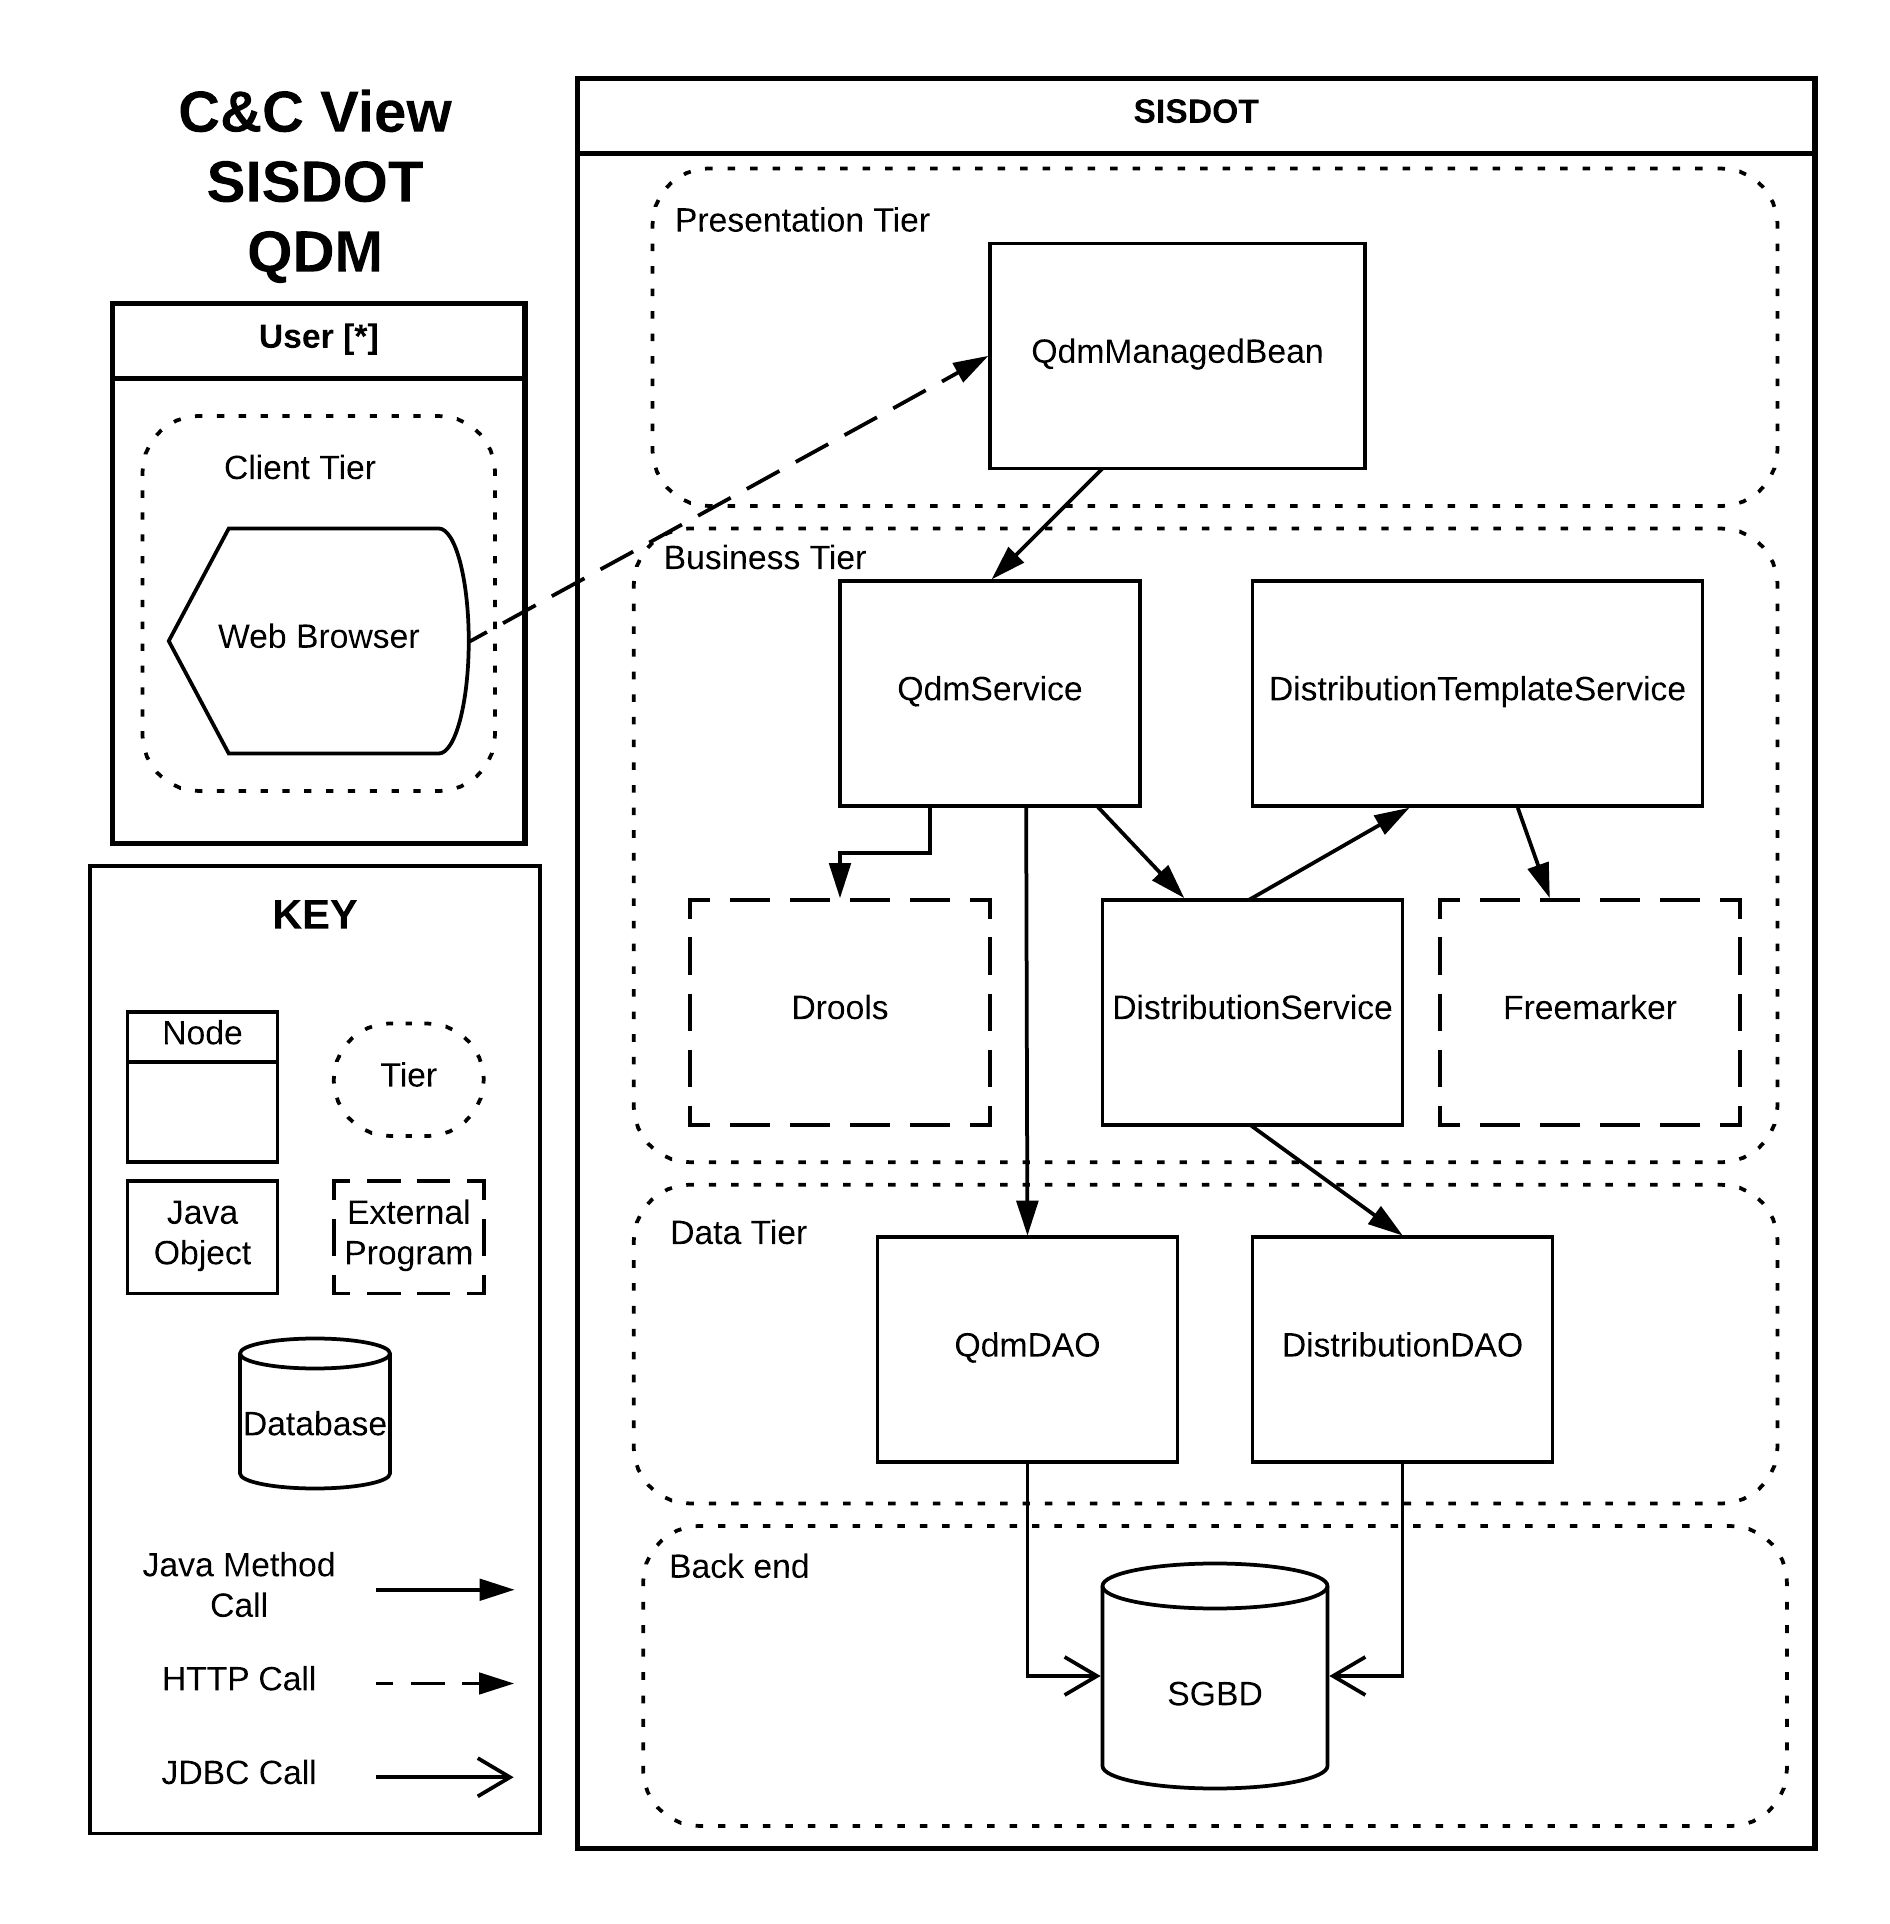
\includegraphics[scale=0.55]{img/runtimeView_qdm.png}
	\caption{Runtime view of the architecture} 
	\label{fig:fig:runtime_qdm}
\end{figure}


\begin{lstlisting}[frame=single, float=*, language=DRL, caption=Example of a \emph{low-level Drools rule}, label={code:drl}]
rule "HLR 1"   	
when
$qc: QuadroDeCargosVO(operational == OPERATIONAL)	
$roles: List( size > 0 ) from accumulate ( 
$dep: DepartmentVO(depId not in (14086, 1130)) from $qc.deps and
$role: RoleVO(function == "ROLE", roleId in (2, 12, 15, 21)) from $dep.roles and  		
QualificationVO(code in ("782", "756")) from $role.qualifications;				
collectList( $role ))	 		
then		 
for(int i=0; i < $roles.size(); i++){       	
RoleVO c = (RoleVO) $roles.get(i);
helper.add(1051000007, c.getFractionId(), c.getRoleId());   
end
\end{lstlisting}

\emph{Considering the user interaction}, a previously authenticated specialist on the distribution of equipment throughout the Brazilian Army, using her web browser, requests the web page that allows the generation of QDMs (one of the main products of SISDOT). 
After selecting the \emph{generic organizational unity} for which a QDM would be generated, the system sends a request to the server. The client tier is responsible for these actions. The request is then received by a component of the presentation tier, more specifically by a \emph{managed bean} that works as a \emph{front controller} (in this case, a JSF controller). 

This controller validates the request data, before sending a new request to the business tier. In the business tier, the service 
that implements the business rules related to the QDM domain object is invoked to start the QDM generation process, which includes actions to (a) transform \callers into the \emph{low-level rules} specified using the Drools Rule Language (DRL), (b) execute these rules to instantiate a business object that represents a QDM, and (c) save this object in the persistence layer (a relational database). 

This process for generating a QDM starts by retrieving a list of previously registered \callers. An \shc, regardless of its type (either based on the full structure of the organization or based on its components), is related to one or more \emph{military materials / equipment} (MEMs) and defines the respective amount that should be assigned to a military unit (which ranges from an organization, a center, a department, a brigade, or even a military function or qualification of a soldier). 

A high-level rule has one or more distribution rules. Each rule has a type, a value, and an associated description. For example, a rule for a department type has the value of the department identifier and the description of the department name. For a better use of the database, avoiding the definition of numerous columns that would inevitably be null for several rule types, we decided to persist the distribution rules of an \shc using JSON (JavaScript Object Notation), which is converted back to an object when it is retrieved. The set of these rules defines exactly who should receive the MEMs specified by the \shc.

One of the factors that motivated the use of a rule based engine was the similarity between \callers and the ``if-then'' rules of these mechanisms.  %whose essential structure is shown in Listing~\ref{code:drlStructure}.
An \shc has a set of conditions that fits the conditional part of a rule (``if'') and has a set of actions (``then'') that, in this case, trigger the distribution of MEMs throughout the expected military unities.

%\begin{lstlisting}[frame=single, caption={Structure of a rule specified in Drools}, label={code:drlStructure}]
%rule "name"
%    attributes
%    when
%        LHS
%    then
%        RHS
%end
%\end{lstlisting}


The list of retrieved \callers contains only Java objects. In order to be able to use the rule engine in a transparent way for the end users (and also for developers in future maintenance scenarios), we decided to use a meta-programming approach, translating these objects into a set of rules (a program in logic programming) that might be used by a rule-based engine. As mentioned before, we decided to use the \emph{Drools rule-based engine} in the context of SISDOT (Figure \ref{fig:fig:runtime_qdm}), mostly because of its integration capabilities with both JEE systems and the Wildfly application server. Accordingly, the \callers are translated into DRL rules (Listing~\ref{code:drl} presents an example of a \emph{low-level Drools rule}). To this end, we use a template engine (FreeMaker) to implement this particular transformation (Figure \ref{fig:fig:runtime_qdm}), using a template that contains the required \emph{markups} for transforming \shc into \emph{low-level} Drools rules. That is, for each \shc, the template engine populates the template, resulting in a DRL rule consistent with the converted \shc.
% A code snippet of the template used for DRL generation can be seen in Appendix A. 

The RHS of the Drools rule of Listing~\ref{code:drl} iterates over all selected military roles (that satisfy the constraints of the LHS). We use a helper class to assign the equipment id (in this case a \emph{rifle} whose id is 1051000007) to the individual roles. Besides providing means to populate a QDM, this helper class also checks some constraints related to the QDM domain model. 
%\begin{figure}[!ht] \centering
%	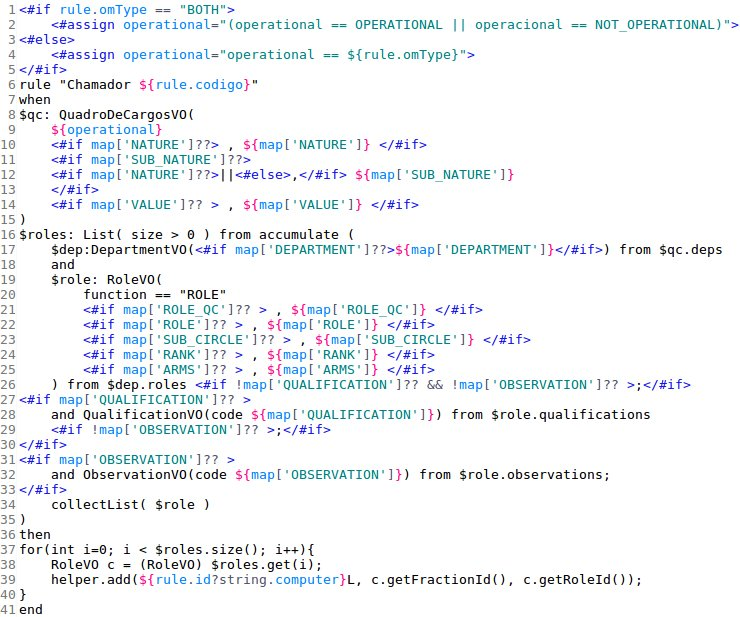
\includegraphics[width=.48\textwidth]{img/artigo_template.jpg}
%	\caption{\it Freemarker template for generating DRL} 
%	\label{fig:template}
%\end{figure}


A QDM is generated for a generic organizational unity (hereafter QC, from \emph{Quadro de Cargos} in Portuguese), selected by the user on the client tier. Therefore, the user-specified QC must be retrieved from the Brazilian Army's enterprise database through a specific Data Access Object (DAO) in the data tier~\cite{alur2003}. From the list of DRL rules, created based on existing \callers, the rule engine is instantiated and these rules are compiled, so that they can be triggered by Drools. The QC domain object is then inserted into the working memory as a fact, an information that is always considered true. The rules are only executed when their conditions are satisfied, based on the specified QC organizational structure. When a rule is valid, that is, it has been activated 
and the \emph{Left Hand Side} (LHS) conditions are valid, the QDM is populated with the MEMs specified in the \emph{Right Hand Side} (RHS) of the rules. Therefore, we generate a complete QDM object after verifying all valid rules (previously registered in the database) for the selected QC. 

After generating a QDM domain object, it is saved on the database and we let the domain expert know of the success of the operation using a simple user interface message. The domain expert can then perform the necessary operations on the generated QDM, including a workflow involving  its edition, homologation, and validation.  



%%%%%%%%%%%%%%%%%%%%%%%%%%%%%%
%% A Domain Specific Language for testing QDM Generation
%%%%%%%%%%%%%%%%%%%%%%%%%%%%%%
\subsection*{A Domain Specific Language for testing QDM Generation}
As explained before, to generate a QDM, a set of \callers must be previously declared. This is a time-consuming task, particularly when using the interface of the system. In order to facilitate the definition of the \callers used in the automated test scripts, we 
decided to implement \hlrdsl---a DSL (Domain Specific Language) that enables us to specify \callers in a clear, objective, and declarative way (and most important, without using the interface of the SISDOT system). 

We implemented \hlrdsl  using Xtext, which generates plugins that allow code editing in both Eclipse and IntelliJ, plus an editor that can be embedded in a web application. This way, a developer writing test scripts might use \hlrdsl to take advantages of the functionality provided by these plugins. To implement a DSL using Xtext, it is first necessary to declare a grammar expressed
using a syntax similar to ANTLR~\cite{parr2013}. Listing~\ref{code:gramatica} presents the grammar of our DSL. From this grammar,the Xtext tool suite generates a lexer, a parser, a set of classes representing the AST (Abstract Syntax Tree), and an editor with several features typically available in IDEs.
% Although Xtext provides an interesting implementation for all these concerns, a language designer is also able to customize several of the Xtext outcomes~\cite{bettini2016}.

%\begin{figure}[!ht] \centering
%	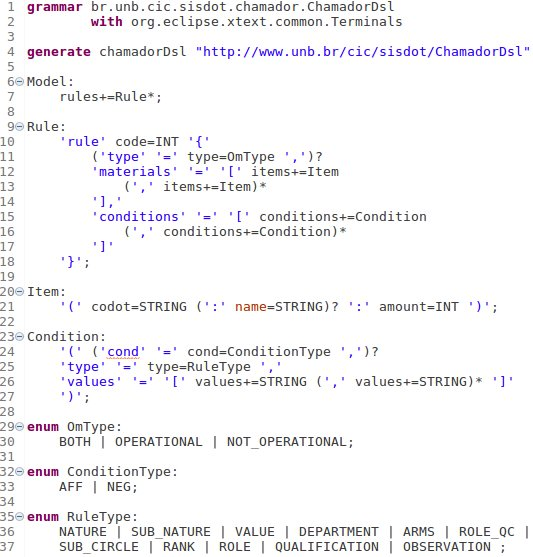
\includegraphics[width=.47\textwidth]{img/artigo_gramatica.jpg}
%	\caption{\it Xtext grammar defining the DSL structure} 
%	\label{fig:gramatica}
%\end{figure}

\begin{lstlisting}[frame=single, language=Xtext, caption={\it Xtext grammar defining the DSL structure}, label={code:gramatica}]
grammar br.unb.cic.sisdot.chamador.HLRDsl 
with org.eclipse.xtext.common.Terminals
generate hlrdsl "http://www.unb.br/sisdot/hlrdsl"

Model:
rules += Rule*;

Rule:
'rule' code = INT '{'
('type' '=' type=OmType ',')?
'materials' '=' '['items+=Item (',' items+=Item)*'],'
'cnds' '=' '['cnds+=Condition (',' cnds+=Condition)*']'
'}';

Item: '(' codot=STRING (':' name=STRING)? ':' amount=INT ')';

Condition:
'(' ('cond' '=' cond=ConditionType ',')?
'type' '=' type = RuleType ','
'values' '=' '[' values+=STRING (',' values+=STRING)* ']'
')';

enum OmType: BOTH | OPERATIONAL | NOT_OPERATIONAL;
enum ConditionType: AFF | NEG;
enum RuleType: NATURE | SUB_NATURE | VALUE | DEPARTMENT | ARMS | ROLE_QC | SUB_CIRCLE | RANK | ROLE | QUALIFICATION | OBSERVATION ;
\end{lstlisting}

Listing \ref{code:dslExample} presents a simple example of a \shc declaration using our DSL. The goal of this rule is to distribute 
the materials (defined in the list of materials construct) for \emph{operational} OMs (see the type construct) and militaries \emph{not working in the specified list of departments} with a set of qualifications and roles. While the definition of this rule 
using our DSL requires 12 lines of code, the corresponding definition of the same rule using a Java test case requires more than 50 lines of imperative code.

Our first test approach consists first in the specification of the required \callers in a \hlrdsl file. Next, the \emph{behavior under test} is detailed as features using the Cucumber~\cite{wynne2017cucumber} framework (we present an example of a feature in Listing \ref{code:cucumber}). After that, the developer details the implementation steps of the features by (a) specifying which \callers(previously declared using our DSL) should be considered in the test execution, (b) specifying which QC the QDM should be generated, and (c) specifying the expected results in terms of the properties of the expected QDM. To this typical scenario, we use a testing  infrastructure that supports several facilities, that aims to increase productivity, such as: database connectivity, auxiliary methods for executing queries in the database, and predeclared rules in the rule engine.

\begin{small}
	\begin{lstlisting}[frame=single, language=DSL, caption={\it Example of a \shc declaration using our DSL}, label={code:dslExample}]
	rule 1 { 
	type = OPERATIONAL, 
	materials = [ 
	("1051000007" : "Rifle" : 1), 
	("1020100011" : "Rifle Carrying Case" : 2)
	], 
	cnds = [ 
	(cond=NEG, type=DEPARTMENT, values=[14086 , 1130]),
	(type=QUALIFICATION, values=[782, 756]), 
	(type=ROLE, values=[2, 12, 15, 21])
	]
	}
	\end{lstlisting}
\end{small}


That is, \hlrdsl simplifies the process of specifying \callers and its primary goal was to assist in test activities. However, after presenting to domain experts some examples of \callers specified using our DSL, we realized that \hlrdsl might also be useful to simulate the specification of rules, allowing a better understanding of the effect of each \shc for building QDMs.


%\begin{figure}[!ht] \centering
%	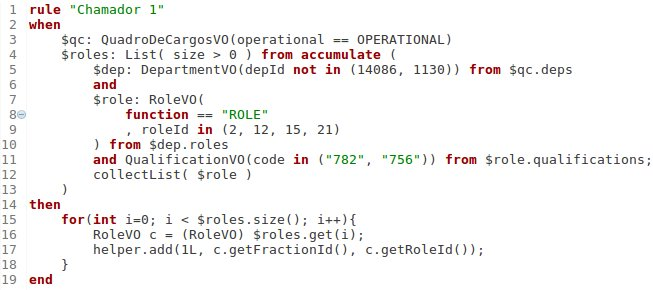
\includegraphics[width=.48\textwidth]{img/artigo_drl.jpg}
%	\caption{\it DRL generated} 
%	\label{fig:drl}
%\end{figure}


Our second test approach automatically generates test cases from our DSL and from a random sample of simple combinations that characterize artificial organizational unities. This \emph{property based approach} involves a custom Maven plugin that currently generates simple test cases, freeing the tester to create only complex tests related to the QDM generation. These test cases are generated from a combination of conditions, for example: one test case only for operational OMs and another for non-operational OMs; a test case for the different kinds of OMs (artillery, infantry, cavalry, aviation and helicopters, general services, and so on), combining with the operational type, such as: operational infantry OMs and non-operational infantry OMs. These combinations are generated for simple cases so that they are easy to verify without the need to manually implement Java test scripts for generating QDMs. 

%\begin{figure}[!ht] \centering
%  \includegraphics[width=.32\textwidth]
%  {img/plugin.jpg}
%  \caption{\it Maven plugin for test generation}
%  \label{fig:pluginExample}
%\end{figure}
% \begin{lstlisting}[frame=single, language=Plugin, caption={\it Maven plugin for test generation}, label={code:plugin}]
% <plugin>
%   <groupId>xxx</groupId>
%   <artifactId>xxx</artifactId>
%   <executions>
%     <execution>
%       <id>execute</id>			
%       <configuration>
%         <seed>10</seed>				
%         <qcs>702311,762314,575311</qcs>				
%       </configuration>
%       <goals>
%         <goal>generate</goal>
%       </goals>
%     </execution>
%   </executions>
% </plugin>	
% \end{lstlisting}

In this second approach, for each of the possible combinations, we generate a \shc that meets the conditions and a cucumber feature that exercises the \shc and compares the expected results declared in the feature. Each \shc is considered during the generation of the QDM to the QCs specified in the maven plugin.% (as shown in Listing~\ref{code:plugin}).
That is, to use this architecture characteristic (here we consider testability as an architecture concern), we ``feed'' the maven plugin with a list of QC codes for which the QDMs should be generated, besides other optional information, which have default values, such as: database connection string, seed to be used in the random selection of values within a combination (e.g., considering 20 different kinds of organizational unities, randomly take 5 for generating the set of combinations), and the output directory 
where the code should be exported. 

%\begin{figure}[!ht] \centering
%  \includegraphics[width=.45\textwidth]
%  {img/artigo_cucumber.jpg}
%  \caption{\it Cucumber feature}
%  \label{fig:cucumber}
%\end{figure}

\begin{lstlisting}[frame=single, language=Cucumber, caption={\it Cucumber feature}, label={code:cucumber}]
Feature: QDM 757311
As a user
I want to generate a QDM from HLRs

Scenario: Test 1
Given QC with code 757311
And HRL: 1, 2
When I generate a QDM
And the results are consistent
Then positions must be populated
| idDep    | idPos   | codot      | amount |
| 6765748  | 10403   | 1051000025 | 1      |
| 6765748  | 10403   | 1020100017 | 1      |
| 6765748  | 10403   | 1020100013 | 1      |
| 6765748  | 10403   | 1051000006 | 1      |
| 6765748  | 21328   | 1051000025 | 1      |
| 6765750  | 10122   | 1051000025 | 1      |    
| 6765793  | 13276   | 1051000025 | 6      |
| 6765796  | 24655   | 1051000025 | 1      |
| 6765796  | 24429   | 1051000025 | 2      |
| 6765798  | 24429   | 1051000025 | 3      |
| 6765798  | 11433   | 1051000025 | 9      |   
And the final result must be:
| codot      | amount |
| 1020100013 | 74     |
| 1020100017 | 74     |
| 1051000006 | 74     |
| 1051000025 | 74     |

\end{lstlisting}

After running the plugin, with the generated code, the tests are executed in a similar way to the test definitions detailed before. The tests run along with the other unit tests declared, whether DSL-based or not.








%%%%%%%%%%%%%%%%%%%%%%%%%%%%%%%%%%%%%%%%%%%%%%
%% Empirical Study
%%%%%%%%%%%%%%%%%%%%%%%%%%%%%%%%%%%%%%%%%%%%%%
\section*{Empirical Study}
\label{sec:case_study} 
For the validation of the proposed architecture we conducted an empirical study, which consists of the evaluation of the main architectural decisions of SISDOT, which relate to the generation of QDMs. The case study aims to answer the following research questions:

\begin{itemize}
	\item \textbf{RQ.1}: Does our proposed approach, based on meta-programming, generate correct QDMs?
	\item \textbf{RQ.2}: Does the use of a DSL reduce the effort necessary to implement the test cases that target QDM generation? 
	\item \textbf{RQ.3}: Does our proposed approach, based on meta-programming, generate QDMs within a satisfactory time-frame?
\end{itemize}

\textbf{RQ.1} deals with the most important concern: correctness regarding the QDM generation. It is intended to demonstrate that the solution not only automatically generates the rules, eliminating the work that the developer would have to implement the solution in Java, but also that the proposed approach leads to the expected QDMs when considering a well defined set of \callers. \textbf{RQ.2} is related to the productivity of the tester and demonstrates how much code the developer have to write when using our DSL, compared to the effort to specify \callers using the Java language in unit test cases. During the activities of requirements elicitation,we identified a softgoal stating the  acceptable time for generating a QDM, which should not be above 5 seconds, when using 1000 \callers. Thus, \textbf{RQ.3} serves to ensure that the QDMs are generated in a satisfactory time.



%%%%%%%%%%%%%%%%%%%%%%%%%%%%%%
%% Data Collection and Analysis Procedures
%%%%%%%%%%%%%%%%%%%%%%%%%%%%%%
\subsection*{Data Collection and Analysis Procedures}
We answer our first question qualitatively. Although this might look like disappointing (under the perspective of empirical methods), we have strong evidences collected from the domain experts that our approach has produced correct QDMs. We believe that this correctness is due to several factors, including the involvement of the domain experts that helped us to full understand the requirements and the expertise of our development team. Nevertheless, the decision of not writing the low-level rules at the source code level, but instead using a program generation approach that has reduced significantly the effort needed to \emph{hand write} 
those rules, has also contributed to achieve this confidence about correctness. 

In a meeting with the domain experts, one of the specialists said: ``I got surprised with the correctness of the solution. In the previous version of the system, we had to have several interactions until we got confident about the correct operation of the \callers''. The first time that we generate QDMs, the process was validated. It is important to note that ``life is not a bed of roses'', and we broke the initial implementation after the introduction of a new, at first not so related feature that, in the end, cut across several classes of the system. We fixed the related issues recently.  

To answer the other two research questions, we collected the following metrics: lines of code (LOC) and execution time. The choice of these two metrics is related to the size of the code, which may indicate higher productivity; and to the fulfillment of the functional requirement that determines the maximum execution time for the generation of QDMs.

\begin{table}[htb!]
	\centering
	\caption{Comparing the number of lines of code need to specify test cases using our DSL and Java}
	\label{table:comparacao}
	\begin{center}
		\begin{tabular}{ccc}
			\toprule
			\textbf{\shc Code} & \textbf{Lines of Code (DSL)} & \textbf{Lines of Code (Java)}     \\ \midrule
			1        & 10  & 26   \\ % \hline
			2        & 10  & 25   \\ % \hline
			3        & 10  & 32   \\ % \hline
			4        & 11  & 52   \\ % \hline
			5        & 15  & 41   \\ % \hline
			6        & 9   & 16   \\ % \hline
			7        & 18  & 21   \\ % \hline
			8        & 12  & 25   \\ % \hline
			15       & 7   & 45   \\ % \hline
			58       & 7   & 58   \\ % \hline
			59       & 17  & 34   \\ \bottomrule
		\end{tabular}
	\end{center}
\end{table}

We use as a benchmark 66 \callers declared in its database. These \callers correspond to real rules used by the Brazilian Army to perform some tests related to the generation of QDMs. We converted each \shc written using JUnit to their correspondent one specified using our DSL. Table \ref{table:comparacao} presents a sample of the collected data. The first column contains the \shc code, the second column contains the number of lines of code to represent the \shc using our DSL, and the third column contains the number of lines of code to represent the same rule in the Java language.

Regarding the runtime metrics, we collected the data using an Intel(R) Core{TM} i7-4790 processor, with 16GB of RAM, running Ubuntu 16.04.4 LTS 64-bit operating system, with 4.15.0-24-generic kernel. We used 16 QCs, chosen to represent the various OM types, natures, and sub-natures. For each QC, we generated QDMs using random sets of \callers with size: 20, 40, 50, 60, 100, 200, 400, 700, 1000, 1500, 2000. Since there were only 66 real \callers already declared, larger quantities contain repeated \callers (which in the end will duplicate the data within a given QDM). The selection of \callers was performed at random, but with the same seed, so that the same sets were used in the generation of QDMs for different QCs. Table \ref{table:tempo} shows a sample of the results obtained with the execution. The first column contains the QC code, and the second column contains the time in milliseconds for the generation of the QDMs using the indicated amount of \callers on the respective column header.

\begin{table}[htb!]
	\centering
	\caption{Time (ms) for generation of QDMs}
	\label{table:tempo}
	\begin{center}
		\begin{tabular}{lllllll}
			\toprule
			\textbf{QC}      & \textbf{60}  & \textbf{100} & \textbf{400}  & \textbf{700}  & \textbf{1000} & \textbf{2000} \\ \midrule
			
			206410  & 184 & 275 & 944  & 1829 & 2279 & 4707 \\ % \hline
			231303  & 197 & 282 & 975  & 1731 & 2541 & 4987 \\ % \hline
			500311  & 201 & 291 & 948  & 1804 & 2289 & 4950 \\ % \hline
			618322  & 175 & 264 & 922  & 1640 & 2412 & 4990 \\ % \hline
			727310  & 173 & 302 & 937  & 1652 & 2466 & 4992 \\ % \hline
			1450311 & 182 & 269 & 890  & 1649 & 2527 & 4785 \\ % \hline
			2203310 & 197 & 263 & 909  & 1619 & 2344 & 4976 \\ % \hline
			5406194 & 176 & 253 & 884  & 1598 & 2393 & 4610 \\ % \hline
			7020003 & 212 & 241 & 922  & 1610 & 2361 & 4470 \\ % \hline
			9131000 & 171 & 252 & 888  & 1609 & 2345 & 4471 \\ \bottomrule
		\end{tabular}
	\end{center}
\end{table}

We exported the collected data to the CSV format, so that we could perform a data analysis using the R environment~\cite{crawley2013}. In the data analysis for \textbf{RQ.2}, which compares the number of lines of code between the two distinct approaches for representing \callers, we created two additional columns: \emph{difference}, which measures the difference in the number of lines of code necessary to specify \callers using Java and our DSL; and \emph{percent of reduction}, which indicates 
how much less code is necessary to specify a \shc using our DSL, when compared to the direct specification in Java code.

\begin{table}[htb!]
	\centering
	\caption{Analysis of DSL and Java comparison data}
	\label{table:analiseComparacao}
	\begin{center}
		\begin{tabular}{llllll}
			\toprule
			& \textbf{Min.}  & \textbf{Median} & \textbf{Mean}  & \textbf{SD}    & \textbf{Max.}  \\ \midrule
			DSL        & 7.00  & 9.00   & 9.67  & 2.81  & 18.00 \\ % \hline
			Java       & 9.00  & 17.50  & 21.76 & 14.68 & 96.00 \\ % \hline
			Difference & 2.00  & 7.00   & 12.09 & 13.94 & 83.00 \\ % \hline
			\%         & 14.29 & 43.75  & 45.23 & 19.84 & 87.93 \\ \bottomrule
		\end{tabular}
	\end{center}
\end{table}

Table \ref{table:analiseComparacao} presents some descriptive statistics of the collected data, containing the following columns: minimum value, median, mean, standard deviation, and maximum value. There is a strong correlation (0.982) between the lines of code in Java and the \emph{difference} measurements. This correlation can be seen in Figure \ref{fig:correlacao}. It is possible to identify that as the size of the Java code grows, the difference for the representation in DSL also increases.

\begin{figure}[htb!] 
	\centering
	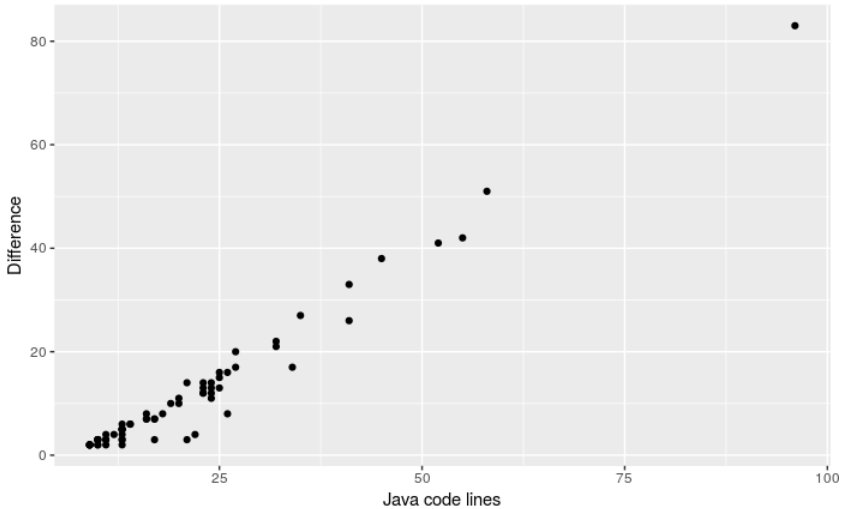
\includegraphics[width=.48\textwidth]
	{img/artigo_correlacao.jpg}
	\caption{\it Correlation between Java and Difference}
	\label{fig:correlacao}
\end{figure}

Figure \ref{fig:geracao} shows the time necessary to generate QDMs for 5 different QCs. For each of them, 6 QMS were generated, with different amounts of \callers, 60, 100, 400, 700, 1000 and 2000.

\begin{figure}[!ht] \centering
	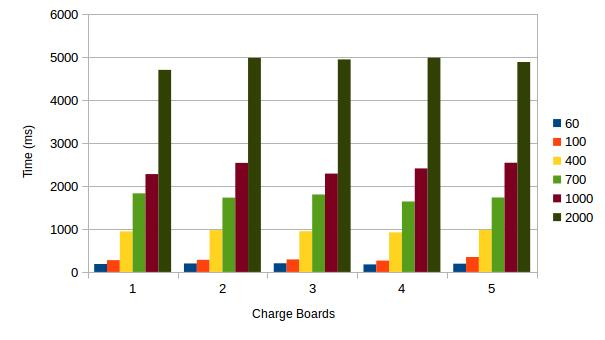
\includegraphics[width=.48\textwidth]
	{img/artigo_geracao.jpg}
	\caption{\it QDM Generation Time (ms)}
	\label{fig:geracao}
\end{figure}



%%%%%%%%%%%%%%%%%%%%%%%%%%%%%%
%% Discussion, Lessons Learned, and Threats to Validity
%%%%%%%%%%%%%%%%%%%%%%%%%%%%%%
\subsection*{Discussion, Lessons Learned, and Threats to Validity}
When analyzing the data related to RQ.2, it was possible to realize that the representation of a \shc using our DSL is on average 45\% smaller than the representation of the same rule in Java. This indicates a possible productivity gain for the developer when writing test cases, since she will have to write a smaller amount of code. In addition, using our DSL, we specify \callers using a declarative approach, which is close to the vocabulary of the problem domain. With respect to the third research question, the limit imposed by the functional requirement of 5 seconds was not exceeded, even when considering 2000 \callers, which is twice the number of \callers expected for the system in production. It is important to notice that these number (5 seconds as time limit and 1000 \callers were collected together with the stakeholders of SISDOT).

The general approach discussed in this paper involves the use of metaprogramming to generate low-level Drools rules from \callers and the use of a DSL to specify \callers during test activities. We have some previous experience using Drools, and, at the beginning of this research collaboration, we realized that the use of a rule based engine (such as Drools), could simplify the computation of QDMs
(one of the main products of SISDOT). Nevertheless, we should try to abstract the use of Drools, mostly due to architectural conformance---we should not introduce new languages during the development of SISDOT. For this reason, we applied a transformational approach, translating Java domain objects into Drools rules at runtime. Perhaps due to the structure of the \callers, the task of implementing this transformational approach was not difficult. We believe that it was the right decision considering the original set of requirements. Surely, a number of uncertainties arise, including: ``will our proposed approach support the expectations of the end-users w.r.t. correctness and time constraints?''. We address this question in our empirical evaluation.

However, we found that testing the process of QDM generation was time consuming, and then we designed a DSL to address the main bottleneck: the specification of \callers either using Java test scripts or the SISDOT user interface (the common way for specifying \callers). Our choice for using Xtext to this end had simplified the entire process for implementing a DSL. Even considering that \hlrdsl is a simple and small DSL, we argue that the set of Xtext tools is really simple and productive, reducing the overall effort to implement the \hlrdsl grammar, parser, and program generator. We could have used other tools and techniques as well, for instance
a metaprogramming approach to support our test activities. However, such approach would not have solved the main problem that motivated us to implement \hlrdsl. In this case, our goal was to design a simple approach for specifying \callers. In the end, \hlrdsl started to be considered an interesting approach for use not only in test activities, but also for simulating QDMs without the need to persist \callers in the production environment. 

Our empirical study presents several limitations. First, we discuss \emph{correctness} based on the results of both integration and acceptance tests, though also considering the opinion of the domain experts that are currently confident that our approach for QDM generation is working properly. Surely, we could have used a more formal approach for discussing correctness, and we postpone this investigation to a future work. Nevertheless, considering the scope of this paper, the feedback from the domain experts and testing outcomes reduce some of ours uncertainties about correctness. 

Second, we only considered 66 real \callers in our study, which served as a basis for measuring the time to generate QDMs. SISDOT is expected to have around 1000 \callers in the production environment. To mitigate the threat related to the small number of available \callers for testing, we considered their repetition when carrying out a performance test of SISDOT. In this way, we expect that the
system would present a behavior similar to the production environment (with respect to performance). The same situation occurs with the comparison of lines of code between the declarations of \callers in DSL and Java. As the number of \callers is relatively small, 
it may not be possible to generalize the results we found.









%%%%%%%%%%%%%%%%%%%%%%%%%%%%%%%%%%%%%%%%%%%%%%
%% Related Work
%%%%%%%%%%%%%%%%%%%%%%%%%%%%%%%%%%%%%%%%%%%%%%
\section*{Related Work}
\label{sec:related}

We addressed the main architectural concerns of SISDOT using well-known patterns for enterprise systems~\cite{enterprise-patterns:book} and software architecture patterns~\cite{pattern-oriented:book}. Moreover, the ideas of using rule based engines to support inference within software systems are also not new~\cite{ORDONEZ2016353,li2012modeling}, and have been particularly explored in the health domain~\cite{mantas2012comparing,li2012modeling,jung2011executing}. For instance, Van Hille et al. present a comparison between Drools and OWL + SWRL for implementing the reasoning procedures of the alert module of an implantable
cardioverter defibrillator. The authors conclude that Drools provides greater expressiveness when compared to the other approach. Our decision to use Drools to implement low-level rules was mostly based on its integration to the JEE platform, instead of its expressiveness.
% We also considered the use of Prolog for at least
% expressing the mechanics of the QDM generation, though
% we postponed this work to a future work.

Dingcheng Li and colleagues report on the use of the Drools engine to model and reason about \emph{electronic health records}~\cite{li2012modeling}. To this end, the authors of this mentioned work implemented a \emph{model-to-model translational approach} that converts the specification of phenotyping algorithms expressed using the Quality Data Model (from the National Quality Forum\footnote{http://www.qualityforum.org/Home.aspx}) into Drools rules. Similarly, Jung et al. present an approach for executing medical logic modules expressed in ArdenML using Drools~\cite{jung2011executing}. They also used a model-to-model approach implemented using XSLT. Our approach could also be characterized as being based on \emph{model-to-model transformations}, since we translate a business entity model (represented as the \callers Java domain objects at runtime) into Drools rules, though using FreeMarker as template engine.
% The work of Ostermayer et al. also advocates
% the use of DSLs + template engines to generate Drools
% rules~\cite{toostermayer2013simplifying}.

Several DSLs have been proposed to support test activities. For instance, Mugridge and Cunningham present the \emph{Fit Framework for Integrated Tests}, which is based on a DSL~\cite{Mugridge:2005:FDS:1051337} The Cucumber framework also uses a DSL for expressing the expected behavior of software features~\cite{Wynne:2012:CBB:2331446}. Here, we designed a small DSL to reduce the effort for setting up a suite of acceptance tests (based on Cucumber) for QDM generation, particularly helping the test team to specify \callers. 









%%%%%%%%%%%%%%%%%%%%%%%%%%%%%%%%%%%%%%%%%%%%%%
%% Final Remarks
%%%%%%%%%%%%%%%%%%%%%%%%%%%%%%%%%%%%%%%%%%%%%%
\section*{Final Remarks}
\label{sec:conclusao}

In this paper we detailed the main design and architectural decisions we use to implement the mechanisms necessary to support the distribution of materials through the Brazilian Army unities. These decisions included the use of a metaprogamming approach to derive high level business rules in rules specific to a rule based system (Drools) and the definition of a DSL that facilitates the declaration of \callers to build test scripts. 

We carried out an empirical study to validate the proposed architecture, based on the evaluation of one of the main scenarios of our logistic system (SISDOT), related to the generation of QDMs. From the results obtained, it was possible to observe a reduction in the average number of lines of code required for the declaration of a \callers using our DSL, in comparison with the representation of the same \shc in Java. Another result of the case study shows that our approach fulfills a non functional requirement that constraints the expected time to generate QDMs. This limit was not exceeded even when using twice the number of \callers expected for the system in production environment.

Although the architecture discussed here considers the specific needs of the Brazilian Army, we believe that logistic systems from other institutions might benefit from our technical decisions as well.







%%%%%%%%%%%%%%%%%%%%%%%%%%%%%%%%%%%%%%%%%%%%%%
%% ACKNOWLEDGMENTS
%%%%%%%%%%%%%%%%%%%%%%%%%%%%%%%%%%%%%%%%%%%%%%
\section*{ACKNOWLEDGMENTS}

We would like to thank the anonymous referees for the valuable comments and suggestions, which have led to several improvements of this paper. This work is partially supported by \textsc{PROMISE-EB}, a software modernization project involving the University of Bras\'{i}lia and the Brazilian Army.









%%%%%%%%%%%%%%%%%%%%%%%%%%%%%%%%%%%%%%%%%%%%%%
%%                                          %%
%% Backmatter begins here                   %%
%%                                          %%
%%%%%%%%%%%%%%%%%%%%%%%%%%%%%%%%%%%%%%%%%%%%%%

\begin{backmatter}

\section*{Competing interests}
  The authors declare that they have no competing interests.

\section*{Author's contributions}
    Text for this section \ldots

\section*{Acknowledgements}
  Text for this section \ldots
  
  
%%%%%%%%%%%%%%%%%%%%%%%%%%%%%%%%%%%%%%%%%%%%%%%%%%%%%%%%%%%%%
%%                  The Bibliography                       %%
%%                                                         %%
%%  Bmc_mathpys.bst  will be used to                       %%
%%  create a .BBL file for submission.                     %%
%%  After submission of the .TEX file,                     %%
%%  you will be prompted to submit your .BBL file.         %%
%%                                                         %%
%%                                                         %%
%%  Note that the displayed Bibliography will not          %%
%%  necessarily be rendered by Latex exactly as specified  %%
%%  in the online Instructions for Authors.                %%
%%                                                         %%
%%%%%%%%%%%%%%%%%%%%%%%%%%%%%%%%%%%%%%%%%%%%%%%%%%%%%%%%%%%%%

% if your bibliography is in bibtex format, use those commands:
\bibliographystyle{bmc-mathphys} % Style BST file (bmc-mathphys, vancouver, spbasic).
\bibliography{bibliography}      % Bibliography file (usually '*.bib' )
% for author-year bibliography (bmc-mathphys or spbasic)
% a) write to bib file (bmc-mathphys only)
% @settings{label, options="nameyear"}
% b) uncomment next line
%\nocite{label}

% or include bibliography directly:
% \begin{thebibliography}
% \bibitem{b1}
% \end{thebibliography}





%%%%%%%%%%%%%%%%%%%%%%%%%%%%%%%%%%%
%%                               %%
%% Figures                       %%
%%                               %%
%% NB: this is for captions and  %%
%% Titles. All graphics must be  %%
%% submitted separately and NOT  %%
%% included in the Tex document  %%
%%                               %%
%%%%%%%%%%%%%%%%%%%%%%%%%%%%%%%%%%%

%%
%% Do not use \listoffigures as most will included as separate files

\section*{Figures}
  \begin{figure}[h!]
  \caption{\csentence{Sample figure title.}
      A short description of the figure content
      should go here.}
      \end{figure}

\begin{figure}[h!]
  \caption{\csentence{Sample figure title.}
      Figure legend text.}
      \end{figure}




%%%%%%%%%%%%%%%%%%%%%%%%%%%%%%%%%%%
%%                               %%
%% Tables                        %%
%%                               %%
%%%%%%%%%%%%%%%%%%%%%%%%%%%%%%%%%%%

%% Use of \listoftables is discouraged.
%%
\section*{Tables}
\begin{table}[h!]
\caption{Sample table title. This is where the description of the table should go.}
      \begin{tabular}{cccc}
        \hline
           & B1  &B2   & B3\\ \hline
        A1 & 0.1 & 0.2 & 0.3\\
        A2 & ... & ..  & .\\
        A3 & ..  & .   & .\\ \hline
      \end{tabular}
\end{table}




%%%%%%%%%%%%%%%%%%%%%%%%%%%%%%%%%%%
%%                               %%
%% Additional Files              %%
%%                               %%
%%%%%%%%%%%%%%%%%%%%%%%%%%%%%%%%%%%

\section*{Additional Files}
  \subsection*{Additional file 1 --- Sample additional file title}
    Additional file descriptions text (including details of how to
    view the file, if it is in a non-standard format or the file extension).  This might
    refer to a multi-page table or a figure.

  \subsection*{Additional file 2 --- Sample additional file title}
    Additional file descriptions text.


\end{backmatter}


\end{document}
